\documentclass{article}
\usepackage{nips12submit_e}
\usepackage[utf8]{inputenc}
\usepackage[T1]{fontenc}
\usepackage{amsfonts}
\usepackage{amsmath}
\usepackage{txfonts}
\usepackage{microtype}
%
\usepackage{color}
\usepackage[colorlinks=true,urlcolor=blue,citecolor=dgreen]{hyperref}
\definecolor{dgreen}{RGB}{0,127,0}
%
\usepackage[backend=bibtex8,style=ieee,sorting=none]{biblatex}
\addbibresource{genopt-confidant.bib}
\defbibheading{bibliography}[References]{\subsubsection*{#1}\markboth{#1}{#1}}
\renewcommand\bibfont{\footnotesize}
\renewcommand\bibinitdelim{\addnbthinspace}
\DeclareFieldFormat{url}{\url{#1}}
%
%\usepackage{booktabs}
\usepackage[hang,raggedright]{subfigure}
\usepackage{tikz}
\usetikzlibrary{shapes.symbols}
\usepackage{wrapfig}
%
\title{Evolutionary Optimization of a Trust-based Routing Policy}
\author{
Zachary Weinberg \\
Carnegie Mellon University (Silicon Valley) \\
Moffett Field, CA 94035 \\
\texttt{zackw@cmu.edu} \\
}
\nipsfinalcopy % Uncomment for camera-ready version
\begin{document}

\maketitle

\begin{abstract}
We present modifications to a standard mesh network routing algorithm,
OLSR, which render it more robust in the face of malfunctioning or
malicious nodes.  Our modifications are based on the CONFIDANT
algorithm, but redesigned for OLSR, and offer a highly tunable set of
“trust functions” specifying policies for sanctions of misbehaving
nodes.  We apply evolutionary optimization to find a good preset for
these trust functions, and discuss the implications of the form of
this preset.
\end{abstract}

\section{Introduction}

\begin{figure}[b]
\centering
\subfigure[Network structure.]{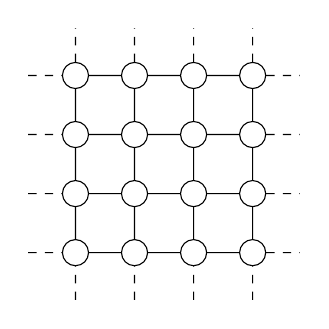
\begin{tikzpicture}
  [every node/.style={shape=circle,minimum size=0.1cm,draw},scale=0.75]
\foreach \x in {1,2,3,4} \foreach \y in {1,2,3,4}
   \node (\x\y) at (\x,\y) {};
\foreach \x in {1,2,3,4} {
  \coordinate (\x0) at (\x,0.2) {} ;
  \coordinate (\x5) at (\x,4.8) {} ;
}
\foreach \y in {1,2,3,4} {
  \coordinate (0\y) at (0.2,\y) {} ;
  \coordinate (5\y) at (4.8,\y) {} ;
}
\draw
  \foreach \x in {1,2,3,4}
    \foreach \ya/\yb in {1/2,2/3,3/4}
      { (\x\ya) -- (\x\yb) }
  \foreach \y in {1,2,3,4}
    \foreach \xa/\xb in {1/2,2/3,3/4}
      { (\xa\y) -- (\xb\y) }
;
\draw[dashed]
  \foreach \x in {1,2,3,4}
    { (\x0) -- (\x1) (\x4) -- (\x5) }
  \foreach \y in {1,2,3,4}
    { (0\y) -- (1\y) (4\y) -- (5\y) }
;
\end{tikzpicture}}%
\hspace{0.5cm}%
\subfigure[Message routing in an intact network.]{\label{f:mesh:route}%
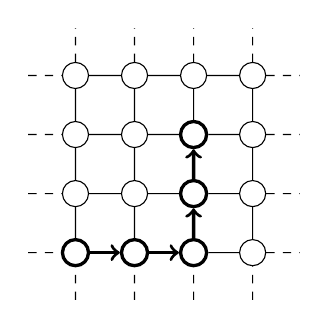
\begin{tikzpicture}
  [every node/.style={shape=circle,minimum size=0.1cm,draw},scale=0.75]
\node [very thick] (11) at (1,1) {};
\node [very thick] (21) at (2,1) {};
\node [very thick] (31) at (3,1) {};
\node []      (41) at (4,1) {};
\node []      (12) at (1,2) {};
\node []      (22) at (2,2) {};
\node [very thick] (32) at (3,2) {};
\node []      (42) at (4,2) {};
\node []      (13) at (1,3) {};
\node []      (23) at (2,3) {};
\node [very thick] (33) at (3,3) {};
\node []      (43) at (4,3) {};
\node []      (14) at (1,4) {};
\node []      (24) at (2,4) {};
\node []      (34) at (3,4) {};
\node []      (44) at (4,4) {};

\draw [very thick,->] (11) -- (21) ;
\draw [very thick,->] (21) -- (31) ;
\draw                                      (31) -- (41)
                 (12) -- (22) (22) -- (32) (32) -- (42)
                 (13) -- (23) (23) -- (33) (33) -- (43)
                 (14) -- (24) (24) -- (34) (34) -- (44) ;

\draw [very thick,->] (31) -- (32) ;
\draw [very thick,->] (32) -- (33) ;
\draw                                      (33) -- (34)
                 (11) -- (12) (12) -- (13) (13) -- (14)
                 (21) -- (22) (22) -- (23) (23) -- (24)
                 (41) -- (42) (42) -- (43) (43) -- (44) ;

\foreach \x in {1,2,3,4} {
  \coordinate (\x0) at (\x,0.2) {} ;
  \coordinate (\x5) at (\x,4.8) {} ;
}
\foreach \y in {1,2,3,4} {
  \coordinate (0\y) at (0.2,\y) {} ;
  \coordinate (5\y) at (4.8,\y) {} ;
}
\draw[dashed]
  \foreach \x in {1,2,3,4}
    { (\x0) -- (\x1) (\x4) -- (\x5) }
  \foreach \y in {1,2,3,4}
    { (0\y) -- (1\y) (4\y) -- (5\y) }
;
\end{tikzpicture}}%
\hspace{0.5cm}%
\subfigure[Node failure requires use of an alternate route.]{%
\label{f:mesh:fail}%
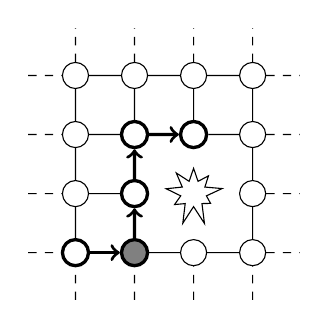
\begin{tikzpicture}
  [every node/.style={shape=circle,minimum size=0.1cm,draw},scale=0.75]
\node [very thick] (11) at (1,1) {};
\node [very thick,fill=gray] (21) at (2,1) {};
\node []      (31) at (3,1) {};
\node []      (41) at (4,1) {};
\node []      (12) at (1,2) {};
\node [very thick] (22) at (2,2) {};
\node [shape=starburst,starburst points=9,
       starburst point height=.3cm,random starburst=1434]
                   (32) at (3,2) {};
\node []      (42) at (4,2) {};
\node []      (13) at (1,3) {};
\node [very thick]      (23) at (2,3) {};
\node [very thick] (33) at (3,3) {};
\node []      (43) at (4,3) {};
\node []      (14) at (1,4) {};
\node []      (24) at (2,4) {};
\node []      (34) at (3,4) {};
\node []      (44) at (4,4) {};

\draw [very thick,->] (11) -- (21) ;
\draw [very thick,->] (23) -- (33) ;
\draw                         (21) -- (31) (31) -- (41)
                 (12) -- (22)
                 (13) -- (23)              (33) -- (43)
                 (14) -- (24) (24) -- (34) (34) -- (44) ;

\draw [very thick,->] (21) -- (22) ;
\draw [very thick,->] (22) -- (23) ;

\draw                                      (33) -- (34)
                 (11) -- (12) (12) -- (13) (13) -- (14)
                                           (23) -- (24)
                 (41) -- (42) (42) -- (43) (43) -- (44) ;

\foreach \x in {1,2,3,4} {
  \coordinate (\x0) at (\x,0.2) {} ;
  \coordinate (\x5) at (\x,4.8) {} ;
}
\foreach \y in {1,2,3,4} {
  \coordinate (0\y) at (0.2,\y) {} ;
  \coordinate (5\y) at (4.8,\y) {} ;
}
\draw[dashed]
  \foreach \x in {1,2,3,4}
    { (\x0) -- (\x1) (\x4) -- (\x5) }
  \foreach \y in {1,2,3,4}
    { (0\y) -- (1\y) (4\y) -- (5\y) }
;
\end{tikzpicture}}%
\caption{Idealized mesh network.}%
\label{f:mesh}
\end{figure}

\subsection{Mesh Networking}

Mesh networks are networks in which every node, or nearly every node,
acts as a router for other nodes' traffic.  Mesh networks are meant to
be robust in the face of communications problems and changing network
topology (e.g.\ from nodes that are moving around), generally can
self-assemble over ad-hoc wireless channels, and are popular where
traditional network infrastructure is absent, nonfunctional, or too
expensive to use.  They face unique difficulties: notably, there may
be no trusted authorities (e.g.\ to register node identities)
whatsoever, there may be no external connectivity, individual links
may be quite slow, and individual nodes may have only a small power
budget.

Figure~\ref{f:mesh} illustrates an idealized mesh network. Each node
has four neighbors, with which it can communicate directly; messages
to more distant neighbors must be relayed, possibly many times, as
shown in figure~\ref{f:mesh:route}.  If a node fails, there are still
alternate routes that can be used; however, as shown in
figure~\ref{f:mesh:fail}, this may involve a different routing
decision at a node which is not a neighbor of the failed node.

Standard mesh-routing algorithms, such as DSR~\cite{s-dsr} (“dynamic
source routing”) and OLSR~\cite{s-olsr} (“optimized link-state
routing”), can cope with node failures, but are not designed to handle
malicious misbehavior.  \emph{Trust-based routing} aims to fill this
gap, by adding reliability assessments to the set of factors
considered when a route is chosen.  We present a trust-based routing
algorithm based on CONFIDANT~\cite{buchegger2002b}, adapted to OLSR
and with evolutionary optimization applied to policy decisions.

\subsection{Threat Model}

The goal of a trust-based routing algorithm is to maintain
connectivity among “honest” participants in the mesh, even in the
presence of “malicious” nodes that are actively trying to subvert it.

We divide malicious node behavior into four broad classes.
\emph{Selfish} nodes originate traffic, participate correctly in the
routing protocol, but overtly refuse to forward any packets for other
nodes.  A standard routing algorithm will treat a selfish node like a
failed node, so they cannot do too much harm.  They do cause other
nodes to do work on their behalf which is not reciprocated, so some
trust-based routing protocols try to detect and punish selfish
behavior, by having other nodes refuse to forward traffic originating
from a selfish node.

One step up from selfish behavior is \emph{sinkhole} behavior. Sinkhole
nodes offer to forward packets, but then discard any packets actually
routed through them.  (Some literature refers to this as selfish
behavior.)  Standard routing protocols may or may not be able to
detect and recover from the presence of sinkholes, but if they can, it
is liable to be slow and inefficient, as it was not an intentional
goal.

Worse yet are \emph{Byzantine} nodes, which attempt to disrupt the
routing protocol in arbitrarily fiendish ways.  One common example of
Byzantine behavior is advertising short routes to nodes that the
malicious node cannot actually reach, and then discarding any traffic
tricked into coming its way.  Standard protocols are not designed to
cope with such trickery, but some TBR protocols attempt it.

Finally, if you do have a TBR protocol, it probably involves control
messages of its own, which identify misbehaving nodes so that other
nodes can avoid them.  \emph{Liar} nodes (so named
in~\cite{buchegger2003}) attempt to subvert this mechanism, causing
honest nodes to be unjustly identified as malicious, or vice versa.

\subsection{CONFIDANT}

The CONFIDANT protocol was proposed by~\textcite{buchegger2002b} as an
enhancement to the standard DSR algorithm.  A subsequent refinement by
the same authors~\cite{buchegger2003} aims to add robustness in the
face of liar nodes.

CONFIDANT nodes \emph{monitor} their neighbors for misbehavior: for
instance, whenever they forward a packet to a neighbor that will be
relayed by that neighbor, they listen to see whether the neighbor
actually carries out the relay.  If it doesn't, they adjust an
internal assessment of the neighbor's reliability; once that
assessment crosses a threshold, they send \emph{alarm} messages to
“friends” (which might be anywhere in the network) and/or back along
the route of the packet that didn't get forwarded.  Alarm messages
cause the recipients to downgrade their own assessment of the
offending node.

\section{Experiment}

For this study we focused on an idealized grid-structured mesh, like
the one shown in figure~\ref{f:mesh}.  Each node has four neighbors,
and are arranged in a square grid pattern, extending for some distance
in all directions.  Unlike the original CONFIDANT experiments, nodes
do not move, and the underlying routing protocol is OLSR rather than
DSR.  OLSR's neighbor and topology discovery algorithm is very easily
modified to take advantage of trustworthiness: there is no need to
transmit “alarm” messages throughout the network.  We implement three
independent responses to a misbehaving node: locally remove it from
the set of relay candidates; downgrade it from a symmetric to an
asymmetric neighbor in \textsc{hello} messages; or cease to pay
attention to its \textsc{hello} messages.  These local actions have
just the desired consequences throughout the network.

%% Position this so it winds up in the upper right hand corner of a page.
\begin{wrapfigure}{R}{130pt}
\hbox to 130pt{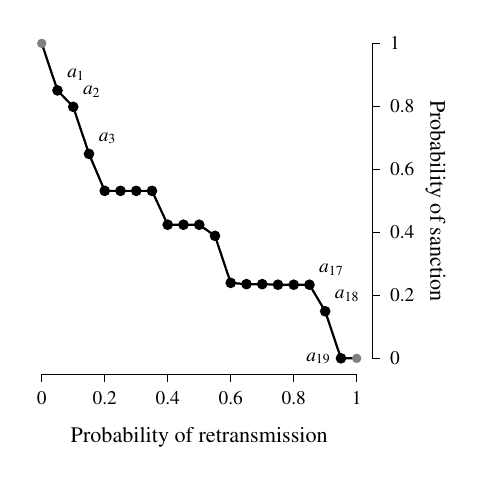
\begin{tikzpicture}[x=4cm,y=4cm]
% axes
\draw
    (1.05,1) -- (1.05,0) (0,-0.05) -- (1,-0.05)
    \foreach \x in {0,0.2,0.4,0.6,0.8,1} {
        (\x,-0.05) -- (\x,-0.075)
        node [below] {\scriptsize \x}
    }
    \foreach \y in {0,0.2,0.4,0.6,0.8,1} {
        (1.05,\y) -- (1.075,\y)
        node [right] {\scriptsize \y}
    }
;
\node at (0.5,-0.25) {\footnotesize Probability of retransmission} ;
\node [rotate=-90] at (1.25,0.5) {\footnotesize Probability of sanction} ;

% control points
\draw [thick] (0,1) -- plot [mark=*,mark size=1.5] coordinates {
  (0.05,0.850634802091)
  (0.10,0.798506348021)
  (0.15,0.649141150112)
  (0.20,0.531740104556)
  (0.25,0.531740104556)
  (0.30,0.531740104556)
  (0.35,0.531740104556)
  (0.40,0.424197162061)
  (0.45,0.424197162061)
  (0.50,0.424197162061)
  (0.55,0.388946975355)
  (0.60,0.239581777446)
  (0.65,0.235548917102)
  (0.70,0.235548917102)
  (0.75,0.233756534727)
  (0.80,0.233756534727)
  (0.85,0.233756534727)
  (0.90,0.149365197909)
  (0.95,0.000000000000)
} -- (1,0);
\fill [color=gray]
      (0,1) circle (0.015)
      (1,0) circle (0.015) ;

\node [above right] at (0.05,0.851) {$\scriptstyle a_1$};
\node [above right] at (0.10,0.798) {$\scriptstyle a_2$};
\node [above right] at (0.15,0.649) {$\scriptstyle a_3$};
\node [above right] at (0.85,0.233) {$\scriptstyle a_{17}$};
\node [above right] at (0.90,0.149) {$\scriptstyle a_{18}$};
\node [left]        at (0.95,0.000) {$\scriptstyle a_{19}$};

\end{tikzpicture}
\hss}%
\caption{A trust function.}\label{f:gene}
\end{wrapfigure}

We considered implementing an OLSR extended link type, which would
allow a node to explicitly notify its 1-hop neighbors of an issue with
a peer; however, in our strict grid-structured mesh, none of the nodes
that such a message would reach are themselves neighbors with the
distrusted node, so it would not be terribly helpful.  We may revisit
this decision when we repeat the experiment with a less-structured
mesh.

\subsection{Trust Functions}

All TBR actions are controlled by “trust functions,” whose general
form is shown in Figure~\ref{f:gene}.  The input to a trust function
is an estimate of the probability that a packet relayed to that
neighbor will be properly forwarded: specifically, it is the upper
limit of the 95\% confidence interval of the mean of a Bernoulli
probability distribution~\cite{wilson1927},
\begin{equation*}
\mathcal{P}_{\text{forward}} =
\frac{r + z^2\slash2 + z\sqrt{z^2/4 + r - r^2\slash n}}
{n + z^2}
\end{equation*}
where $n$ is the total number of packets this node has sent to a
neighbor to be forwarded, $r$ is the number of those packets that the
neighbor was observed to retransmit, and $z$ is the $1-\alpha/2$
quantile of the standard normal distribution (in this case,
$z\approx1.96$).

The output from a trust function is the probability that a sanction
should be imposed.  There are three trust functions, one for each of
the three sanctions listed above; whenever a node has to decide
whether to impose one of the sanctions, it chooses a random number
from the range $[0,1)$, and imposes the sanction if the appropriate
trust function's output is greater than or equal to the random number.

Together, the trust functions comprise the genotype to be optimized.
Each dot in figure~\ref{f:gene} is a control point for a
piecewise-linear interpolation, and the y-coordinates of the
intermediate points are the genes.  The function is constrained to be
nonincreasing overall, i.e. $1 \ge a_1 \ge a_2 \ge \cdots \ge a_{19}
\ge 0$.  This constraint was implemented as a genotype-to-phenotype
transformation.  The evolutionary optimizer worked on a set of
\emph{differences}, $\delta_i = a_i - a_{i-1}$, which could take any
value in the range $[0,1]$; at the beginning of each simulation, the
$a_i$s were recovered from the $\delta_i$s and the overall function
rescaled to the unit interval.

\subsection{Test Scenarios}

\begin{figure}[b!]
\centering
\begin{tabular}{c@{\qquad}c}
50 sinkholes&100 sinkholes\\
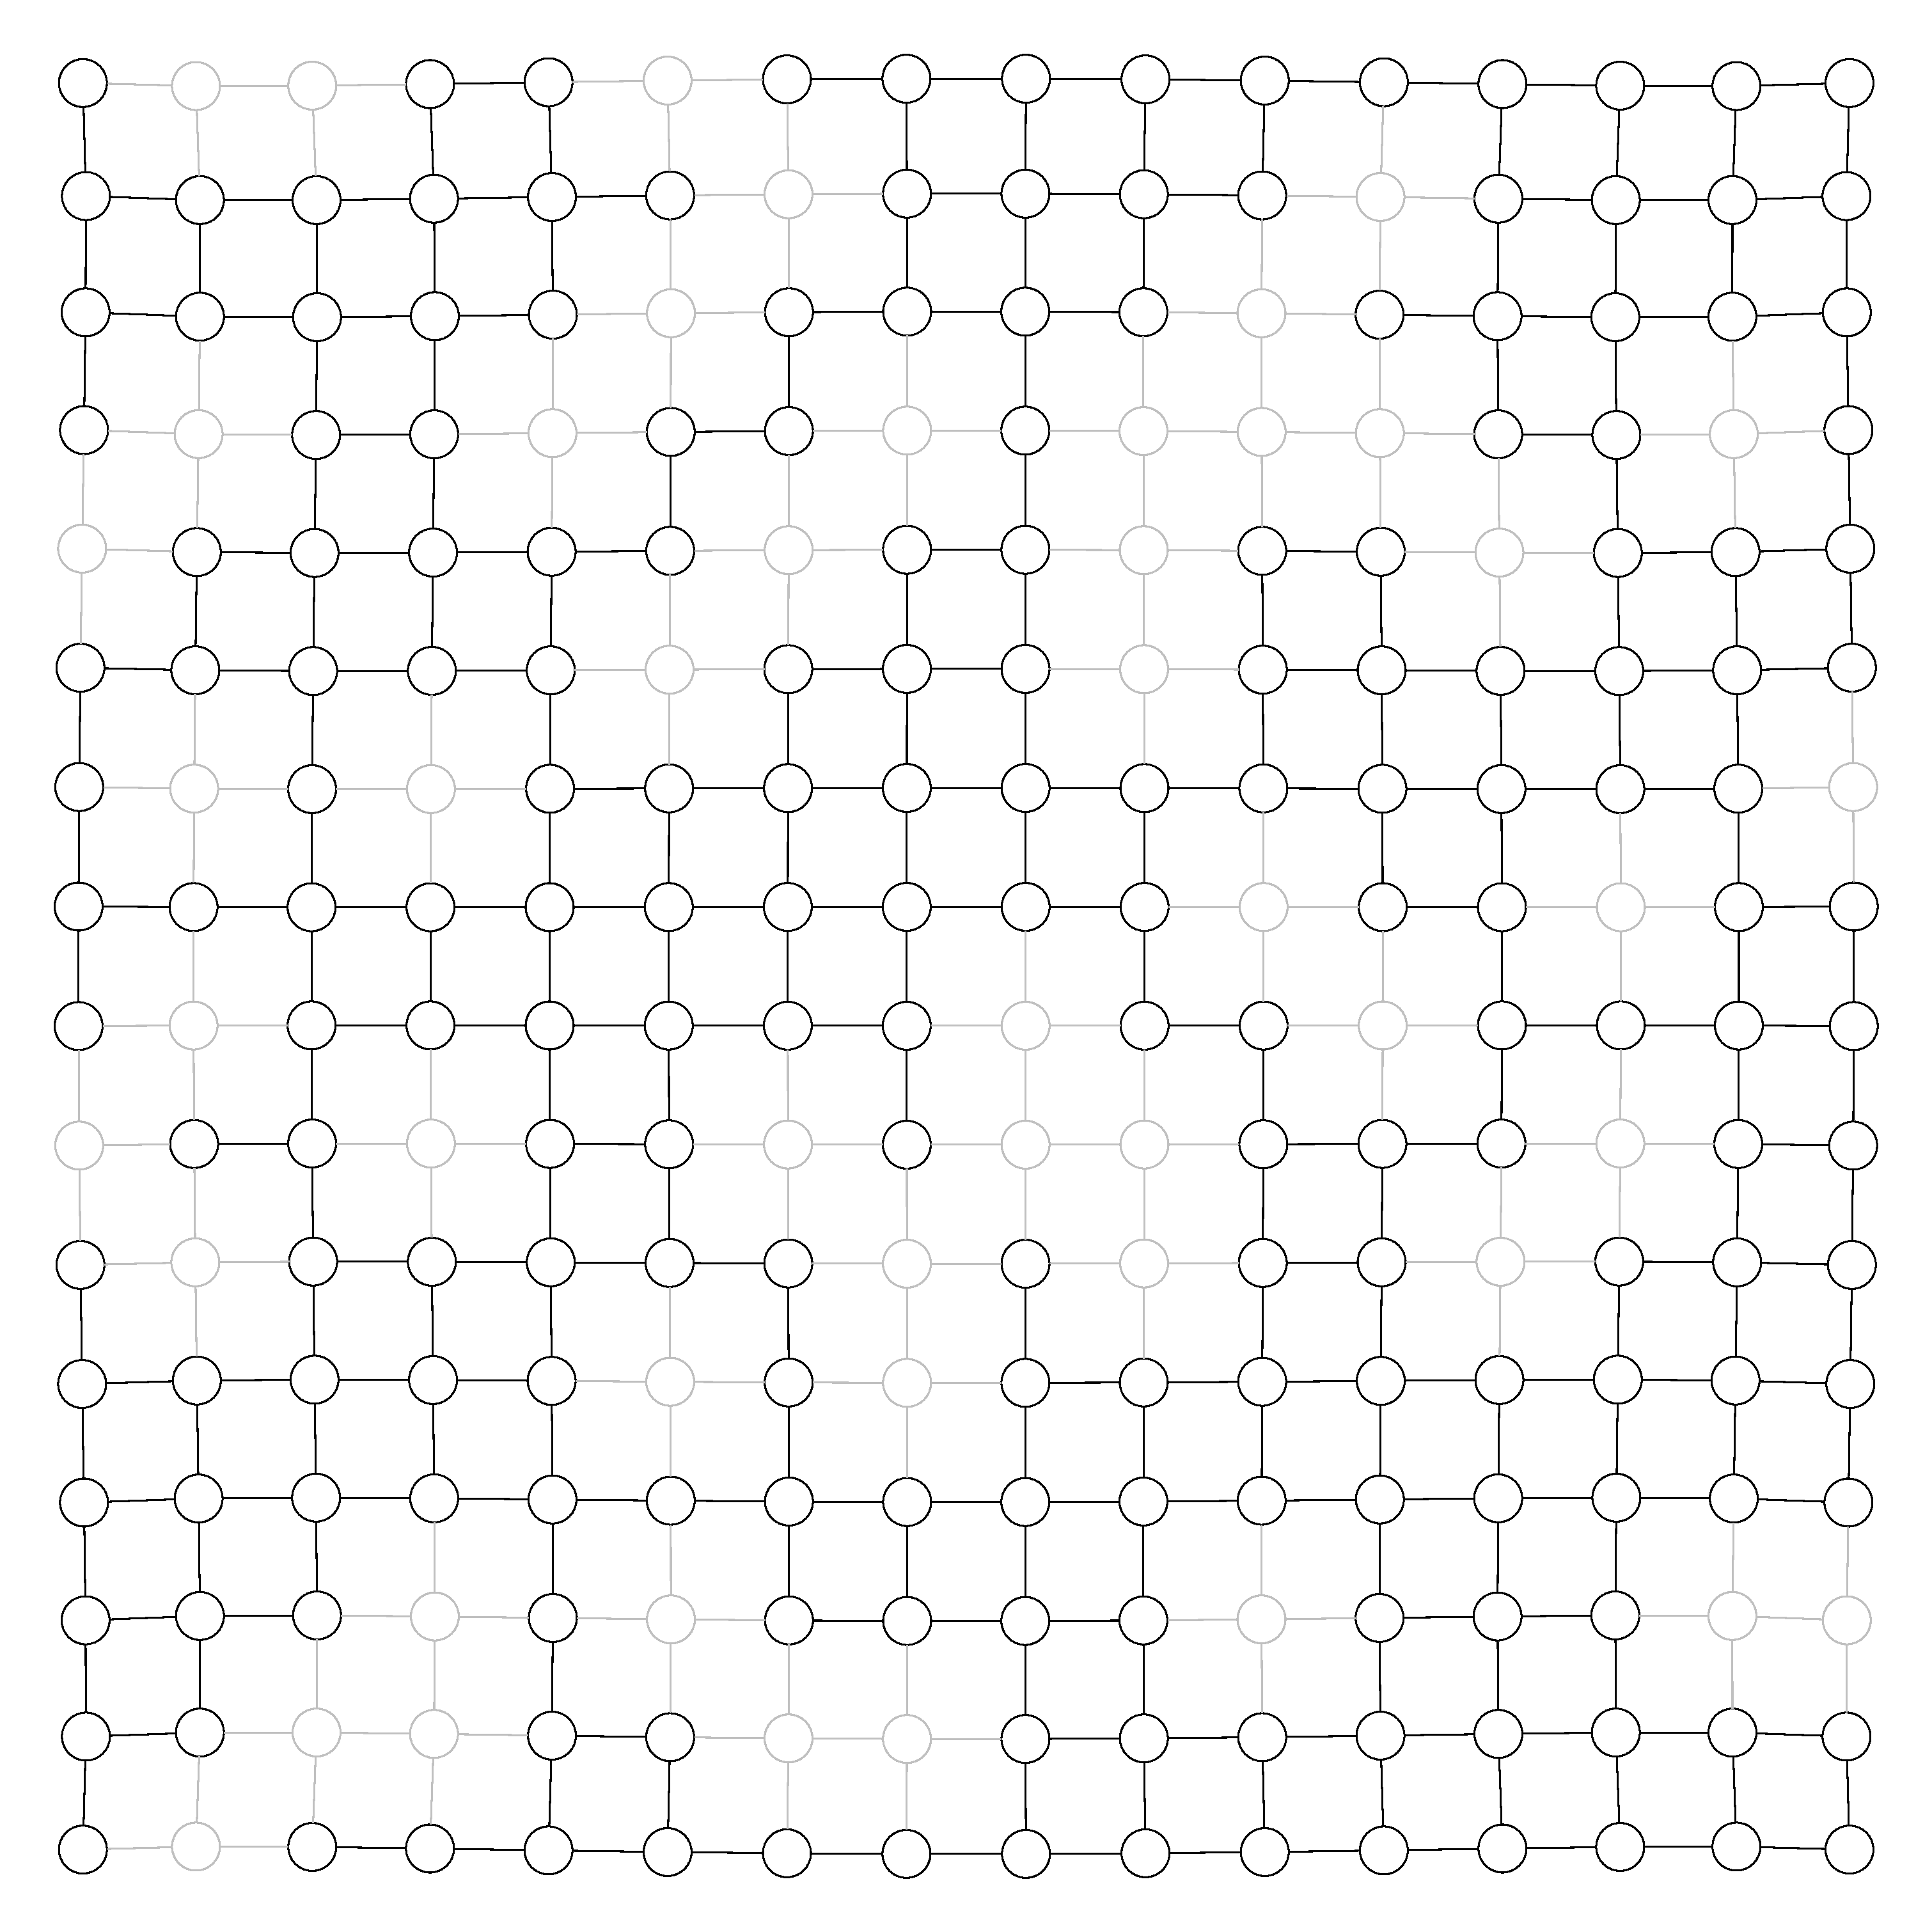
\includegraphics[width=2in]{figures/fifty}&
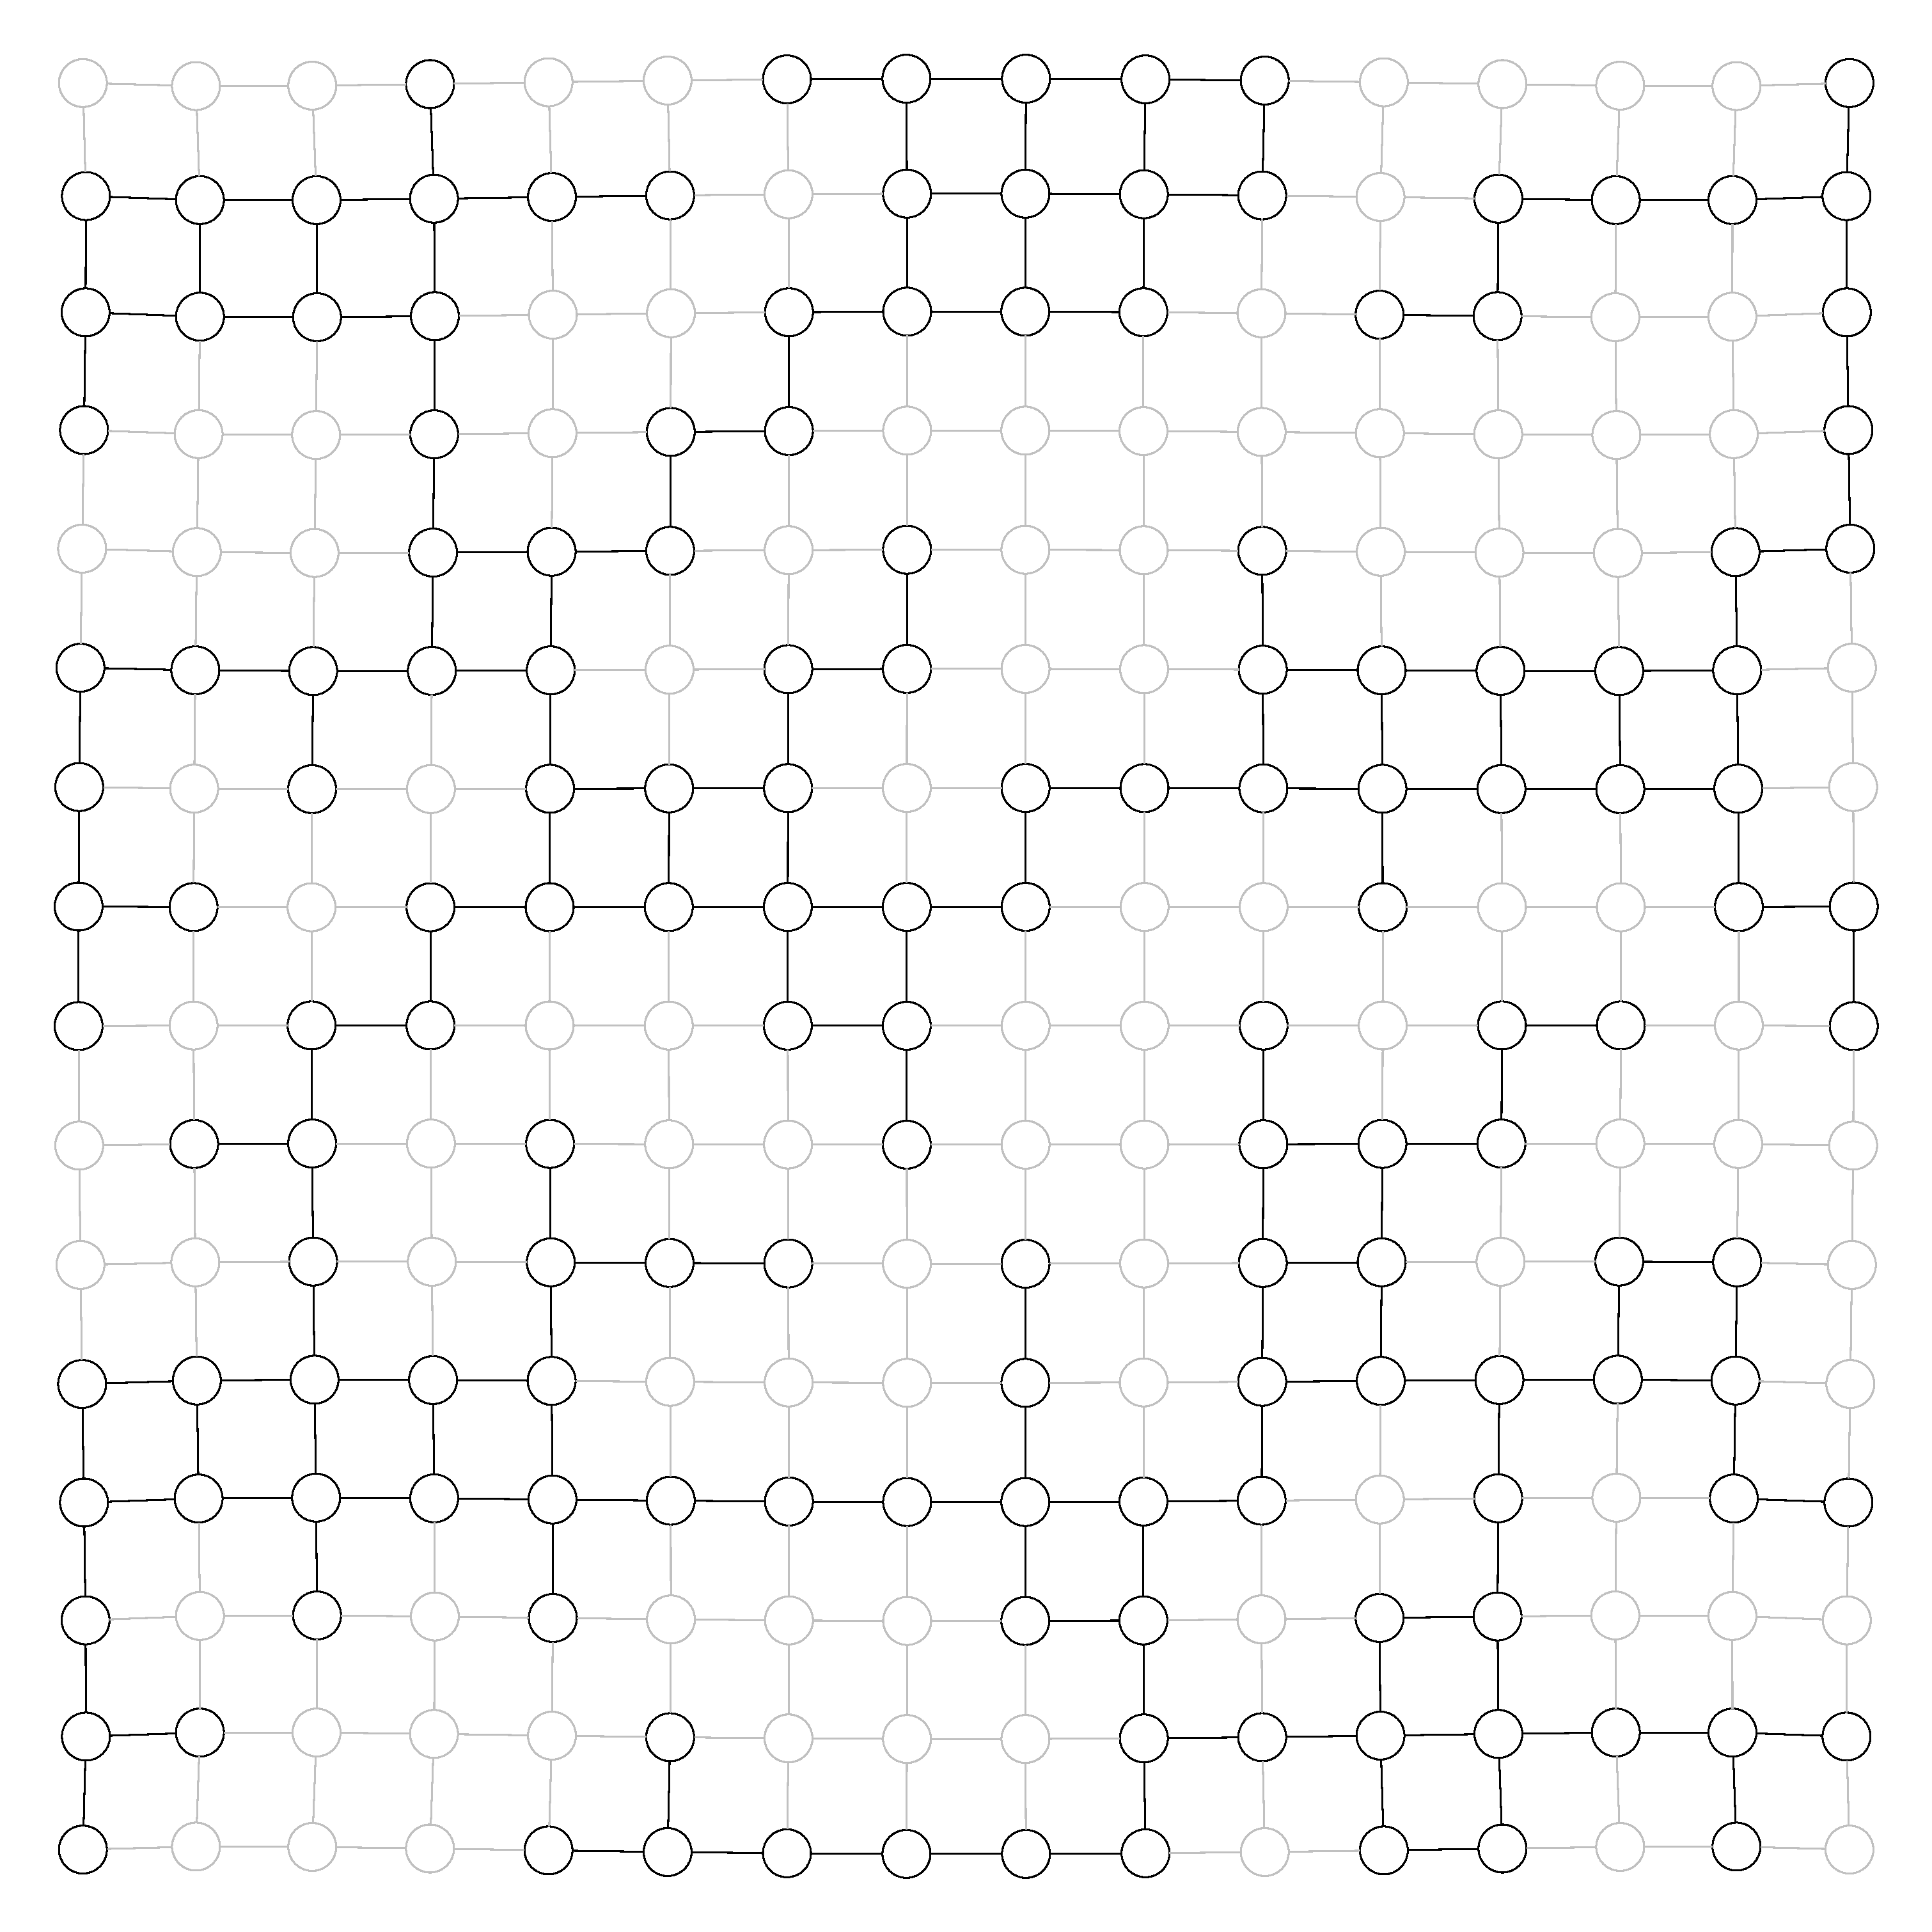
\includegraphics[width=2in]{figures/hundred}\\
\end{tabular}
\caption{Two example challenge networks.  Gray nodes are
  sinkholes. Black nodes generate and receive traffic.  The black
  nodes are never partitioned into two or more disconnected
  clusters.}\label{f:chal}
\end{figure}

We generated 283 \emph{challenge} networks, each a $16 \times 16$
grid-structured mesh, with the only difference being the position and
number of nodes that would behave as sinkholes.  Within each challenge
network, each node is either always a sinkhole, or always a
well-behaved traffic generator and receiver.  Figure~\ref{f:chal}
shows two such networks.  193 of the challenges form a “ramp” from
zero to 192 sinkholes, each possible number of sinkholes represented
once.  The other 90 present alternative arrangements of between 64 and
128 sinkholes (inclusive).  In all cases, sinkhole positioning was
random, but constrained to ensure that the well-behaved nodes could
all still contact each other via a chain of relays all of which were
well-behaved.

We simulated these networks using NS-3~\cite{z-ns3}.  In real life
this kind of mesh would probably communicate by radio, and depending
on local conditions, individual nodes' transmissions might reach more
than one hop away.  For the sake of simulation speed, we did not model
the physical or MAC layers at all; we provided each node in the
simulation with a point-to-point, null-modem connection to its
neighbors.  Furthermore, misbehavior monitoring was faked; the
simulator notified the previous hop in a relay chain of the
send/discard decision taken by its peer.  We only simulated and
monitored for non-forwarded traffic, not any of the other types of
misbehavior listed in~\cite{buchegger2002b}.

During each simulation run, the well-behaved nodes would all
continuously generate fixed-length packets (1024 bytes of UDP payload)
at a rate of ten per second.  Each packet was sent to a different
randomly-chosen destination; any node might attempt to communicate
with any other well-behaved node, but the probability fell off with
the Manhattan distance between the two.  Sinkhole nodes were never
chosen as packet destinations and did not generate any traffic
themselves.  Each simulation ran for 60 seconds of simulated time, and
we measured the goodput per node: that is, bytes per second of UDP
payload successfully delivered to their ultimate destination, not
counting control messages.  Pilot testing indicated that the
simulations took approximately 20 seconds to reach a steady state, so
we discarded the first 30 seconds of data from each simulation.

\subsection{Fitness Assessment}

Ahead of time, for each challenge network, we measured the mean goodput
achieved by unmodified OLSR with all the sinkholes in place, and the mean
goodput achieved by unmodified OLSR if the sinkholes were all replaced
by \emph{selfish} nodes (that is, nodes that overtly refuse to relay
traffic).  Since OLSR has built-in selfish node avoidance, these
baseline scenarios produce worst-case and best-case behavior from the
network, respectively.  We defined the basic fitness of any given
trust function on a particular challenge as
$$
f(g;w,b) = \frac{g - w}{b - w}
$$
where $g$ is the mean goodput measured with that trust function in
place, and $w$ and $b$ are the worst-case and best-case baseline mean
goodput for that challenge.  We also imposed weak penalties for high
variance in goodput, and for over-aggressive sanctions (too many large
$a_i$).

\begin{wrapfigure}[20]{r}{2.5in}
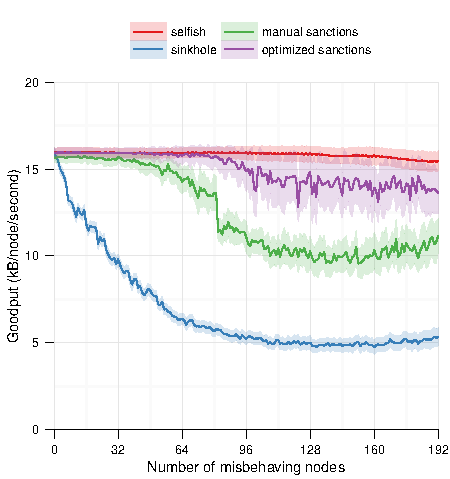
\includegraphics[width=2.5in]{figures/monrampg}
\caption{Goodput achieved by baseline OLSR and our improved
  algorithm.  Ribbons indicate variance.}\label{f:results}
\end{wrapfigure}

Each simulation run required approximately five minutes of wall-clock
time on the hardware available, so we were only able to run
evolutionary optimization against a small population (40 individuals)
for a short interval (50 generations), and we did not have time to
investigate the space of tunable parameters; we simply used the
defaults suggested by the author of ALPS~\cite{z-alps1,z-alps2} for a
single-layer population.  (ALPS was used for convenience rather than
for its more sophisticated features.)  Despite this, the optimizer
achieved a significant improvement over baseline OLSR and over
hand-chosen trust functions, as we will describe below.

\section{Results and Discussion}

Figure~\ref{f:results} shows the worst-case (blue) and best-case (red)
baseline goodput for each of the “ramp” challenges; goodput achieved
on the same set of challenges by a manually-chosen set of trust
functions (green) and goodput acheived by the best individual after 50
generations of evolutionary optimization (purple).  The manually
chosen trust functions recover most of the available goodput for small
numbers of sinkholes, but not all of it, and their performance begins
to deteriorate at about 32 sinkholes (though it is still much better
than no TBR at all).  The optimized functions, by contrast, achieve
goodput indistinguishable from the best-case baseline out to 64
sinkholes, and are much better than the manually chosen functions all
the way to 192 sinkholes, albeit with much larger variance.

\begin{figure}
\centering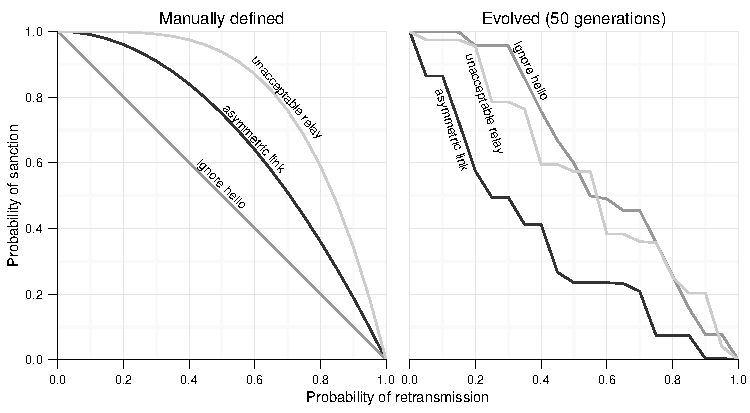
\includegraphics{figures/best-50g}
\caption{Manual and best evolved trust functions.}\label{f:tfopt}
\end{figure}

Figure~\ref{f:tfopt} compares these two sets of trust functions.  The
manually chosen functions were designed on the theory that
`unacceptable relay,' `asymmetric link,' and `ignore hello' formed an
escalating series of sanctions, each being a more aggressive action
than the one before it; therefore, the lightest sanction should be the
most likely.  The evolved functions, by contrast, apply the `ignore
hello' and `unacceptable relay' sanctions with roughly the same
probabilities, somewhat more aggressively than the manual functions
did, and the `asymmetric link' sanction less often.  This suggests
that the latter is not an effective sanction, and the former two are
in some sense the same thing.  This may be because the additional
consequences of `ignore hello' and `asymmetric link' (beyond that of
`unacceptable relay') are not evident in a scenario where sinkholes
don't themselves generate traffic.

\section{Future Work}

A high priority for future work is to investigate less rigidly
structured network topologies, and topologies with more 1-hop
neighbors.  The NS-3 simulator supports a detailed 802.11b wireless
PHY and MAC model, which could easily replace our collection of
point-to-point links, facilitating both greater realism and more
complex network layouts.  (We did not do this in the present work
largely for performance reasons.)  We also plan to investigate newer
ad-hoc routing protocols, such as B.A.T.M.A.N.~\cite{s-batman} and
Babel~\cite{s-babel}.

In view of the form of the evolved trust function, more realistic
application traffic is also highly desirable.  Particularly, sinkholes
should not be wholly passive: they should generate traffic of their
own.  This of course raises the question of whether the network
\emph{should} route traffic on behalf of known bad actors; the answer
may depend on the network's purpose.  Sinkholes should also not always
misbehave.  A genuinely malicious actor would attempt to conceal their
infiltration of the network, after all.

In order to achieve robustness against more sophisticated malicious
nodes (Byzantines and Liars) nodes need to be able to detect more
classes of misbehavior; in particular, bogus route advertisements can
produce significant disruption.  B.A.T.M.A.N. and Babel include a
degree of protection against incorrect
advertisements~\cite{abolhasan2009}, so they would be better baselines
to use.

\section{Related Work}

CONFIDANT is only one of several trust-based routing algorithms in the
literature.  Some of particular interest include:
\textcite{anderegg2003} presents a game-theoretic analysis of the
behavior of nodes which are selfish out of economic self-interest,
e.g.\ because forwarding every packet they are asked to forward is too
much of a drain on their batteries.  They propose a mechanism to pay
these nodes for their efforts, bringing individual nodes' incentives
in line with what is best for the network at large. Of course this
only helps as long as all selfish nodes' motives are economic, and it
is not clear how nodes are to convert payments into battery charge.

\textcite{komathy2008} model packet-dropping attacks as an instance of
the classic game-theory problem Iterated Prisoner's Dilemma, and use
genetic optimization to improve honest nodes' strategies for choosing
which neighbors to use as relays.  Each node only knows about its
neighbors, which is natural given the base routing protocol in use
(AODV, which is hop-by-hop).  We see this work as complementary to our
own: it would be interesting to incorporate information about more
distant peers into this kind of strategy optimization.  For instance,
it does no good to forward a packet to a reliable peer if that peer's
further neighbors are all untrustworthy.

\textcite{hallani2009} use “fuzzy logic” to assess the overall
reliability of routes and avoid routing through nodes that are
unreliable.  Nodes need only maintain trust assessments of their
neighbors; end-to-end reliability of each potential route is computed
during the route-setup process inherited from AODV.  This is an
elegant approach which avoids nearly all extra traffic overhead (route
setup packets are slightly larger); however, liar nodes may be able to
cause significant disruption.

\textcite{ayday2010} point out that the “watchdog” mechanism advocated
by CONFIDANT (at least in the simple, just-listen-for-retransmissions
incarnation actually implemented by \citeauthor{buchegger2002b} and
us) is easy for a Byzantine node to fool, for instance by generating
retransmissions that are powerful enough to be heard by the watching
node but not enough to be heard by the next hop.  They advocate
combining the “watchdog” mechanism with data from end-to-end ACKs
(which have their own problems, of course: for instance, they could be
forged) and also present a sophisticated game-theoretic model of
interactions among many nodes in the network.

All of the above protocols operate in a \emph{flat} network, where all
the nodes are equal.  \textcite{safa2010} instead consider a dynamic
two-level hierarchy, where each node belongs to a “cluster” and
delegates long-distance routing decisions to its “cluster head.”
(Cluster heads do not necessarily act as \emph{relays} for any given
route; they just decide what the routes are.)  Each cluster chooses
its head from among all its members, and can reassign that role at any
time.  Apart from this wrinkle, the protocol is much the same as
in~\cite{hallani2009} (the details differ).  The major advantage of a
hierarchical network is that only the cluster heads need to send and
receive route setup traffic, which reduces overhead.  Unfortunately,
since the structure is so different, it is difficult to compare with
any of the others.

\printbibliography

\end{document}
